%------------------------------------------------------------------------------------------------
The figure shows a crane whose cab \basis{A} supports a boom \basis{B} that swings
a wrecking ball $C_o$.
%\\[0.0pc]
Sets of \dextral ~orthogonal unit vectors (\basisVectors{n}), (\basisVectors{b}), and (\basisVectors{c})
are defined as shown.
%This is the same setup from your homework.
%
\\[0.5pc] The position vector from $N_o$ to $C_o$ is
$\posvec{N_o}{C_o} \equals[\;] x~\uvecx{n} \plus[\;] L_B ~\uvecx{b} \minus[\;] L_C ~\uvecy{c}$.


\begin{minipage}{0.52\textwidth}
%\\[0.5pc]
The angular velocity of \basis{B} in \basis{N} is
$\angvel{B}{N} \equals[\;] \thetadot_B ~\uvecz{b}$.
\\[0.25pc] The angular velocity of \basis{C} in \basis{N} is
$\angvel{C}{N} \equals[\;] \thetadot_C ~\uvecz{c}$.

{\small
\vspace{0.5pc}
\begin{tabular}{|l|c|c|}
          \hline Quantity                                                   & Symbol     & Type
\\[0.0pc] \hline \uvecx{b} distance between $A_B$ and $B_C$      & $L_B$ & Constant
\\[0.0pc]        \uvecy{c} distance between $B_C$ and $C_o$      & $L_C$ & Constant
\\[0.0pc] \hline \uvecx{n} distance between $N_o$ to $A_B$       & $x$ & Variable
\\[0.0pc]        angle between \uvecx{n} and \uvecx{b} about \uvecz{n}      & $\theta_B$ & Variable
\\[0.0pc]        angle between \uvecy{n} and \uvecy{c} about \uvecz{n}      & $\theta_C$ & Variable
  \\[0.0pc]\hline
\end{tabular}}

\end{minipage}
\hfill
\begin{minipage}{0.48\textwidth}
\flushright
\vspace{-2.0pc}
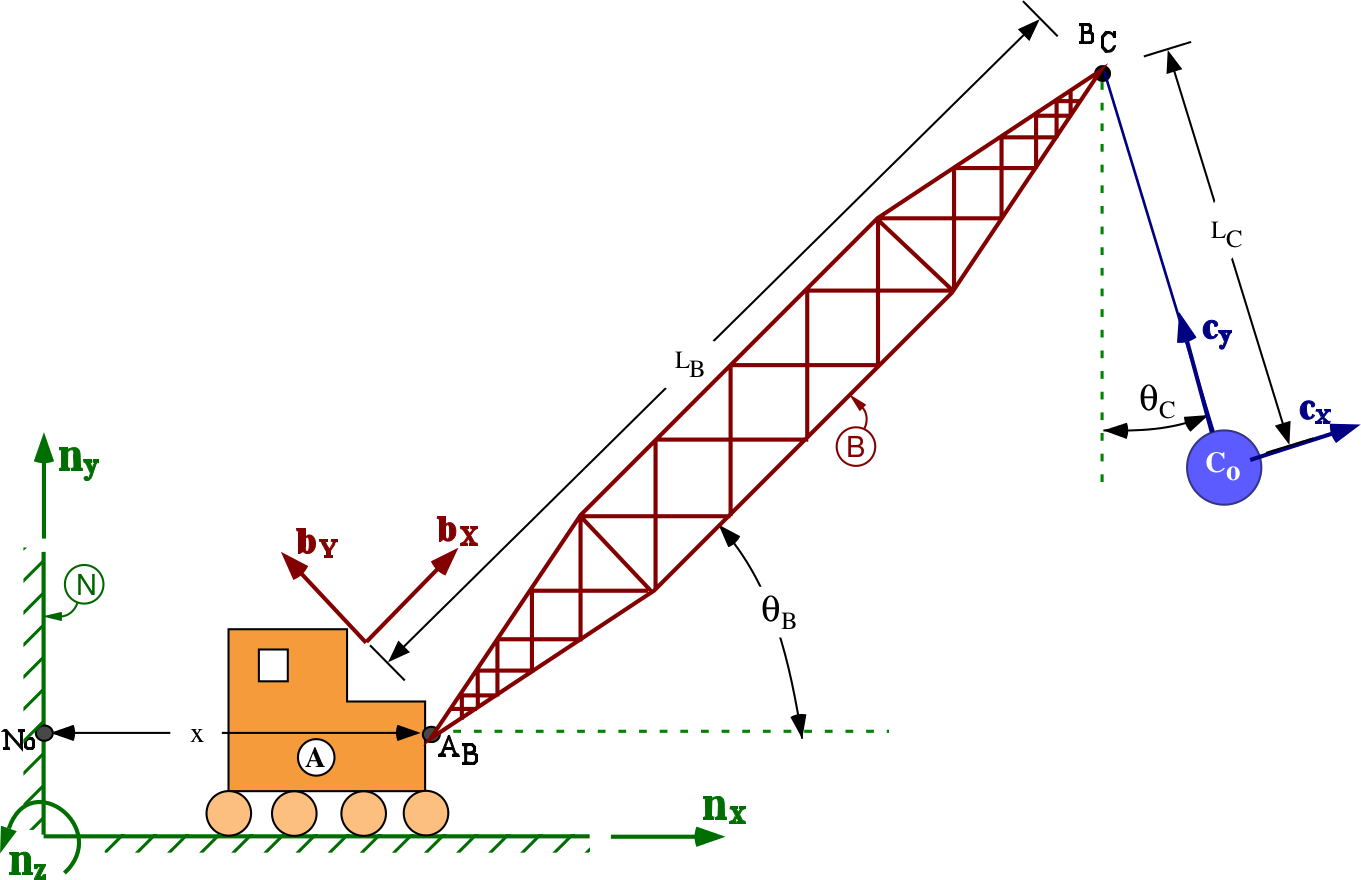
\includegraphics[width=\textwidth]{crane_transparent.png}
\end{minipage}

\begin{enumerate}
%\item Determine the angular velocity of \basis{B} in \basis{N}.
%\\[2.0pc]
%\item Determine the angular velocity of \basis{C} in \basis{N}.
%\\[2.0pc]
%\item Determine the angular velocity of \basis{C} in \basis{B}.
%\\[4.0pc]
\item Express the velocity of $C_o$ in \basis{N} in terms of symbols in the table
and their time derivatives.
\\[0.5pc] $\vel{C_o}{N} \equals[\;]$
\\[11.0pc]
\item Express the acceleration of $C_o$ in \basis{N} in terms of symbols in the table
and their time derivatives.
(It is probably easiest to just differentiate your result from (a),
but you can also use the fact that $\accel{Bc}{N} = \ddot{x}~\uvecx{n} + L_B \thetaddot_B ~\uvecy{b} - L_B \thetadot_B^2 ~\uvecx{b}$ and observe that $B_C$ and $C_o$ are both fixed in \basis{C}.)
\\[0.5pc] $\accel{C_o}{N} \equals[\;]$
\\[11.0pc]
%\item \simpleRotationZ{n}{b}{\theta_B} \simpleRotationZ{n}{c}{\theta_C}
\end{enumerate}